% 第三章 任意构型 Hopfion 的理论模型与构建
\chapter{任意构型 Hopfion 的理论模型与程序化构建}

\section{Hopfion 理论模型回顾}

微磁学模拟对初始磁化分布的质量极为敏感,这一点在探究磁性 Hopfion 的稳定性与动力学时尤为突出。对于拓扑荷 $Q_H=1$ 这类较为基础的情形,Sutcliffe 模型给出的解析解已能提供可靠的起始态;然而一旦涉及更高阶拓扑荷或空间取向更为复杂的结构,则需依赖于基于环面坐标系的理论框架\cite{guslienko2025magnetic}。本文的定位并非提出新的解析解,而是将前人建立的局域旋转矩阵与环面坐标映射理论——原本停留在纯数学描述层面——转译为可被微磁学仿真直接调用的代码工具。围绕这一目标,本章介绍一套面向任意拓扑荷、同时兼容反铁磁(AFM)交替背景的初始态生成脚本的实现思路,并在此基础上给出配套的三维可视化解调方法,为后续仿真研究铺设基础。

\par\noindent\textbf{磁化场的旋转矩阵表示}\par\nobreak
从连续场理论的视角看,Hopfion 本质上是嵌入于均匀磁化背景中的一类三维拓扑孤子。取均匀背景磁化为 $\mathbf{m}_0 = \hat{z}$,则任意复杂构型 $\mathbf{m}(\mathbf{r})$ 都可以通过一个与坐标相关的局部旋转矩阵 $\hat{R}(\mathbf{r})$ 作用于该背景获得,即 $\mathbf{m}(\mathbf{r}) = \hat{R}(\mathbf{r}) \mathbf{m}_0$。

超球面 $S^3$ 的四元数参数化引入向量 $n_\alpha = (n_1, n_2, n_3, n_4)$,满足归一化条件 $\sum n_\alpha^2 = 1$。由 $n_\alpha$ 的各分量可构造出局部旋转矩阵:
\begin{equation}
    R_{ik} = \delta_{ik} + 2(n_i n_k - n^2 \delta_{ik}) - 2\varepsilon_{ikl} n_l n_4
\end{equation}
其中,下标 $i, k, l \in \{1,2,3\}$,$\mathbf{n} = (n_1, n_2, n_3)$,$n^2 = n_1^2 + n_2^2 + n_3^2$,$\varepsilon_{ikl}$ 为完全反对称张量。由此,三维空间中的磁化场分量可化简写为:
\begin{equation}
    \mathbf{m} = (1 - 2n^2)\hat{z} + 2n_z \mathbf{n} + 2n_4(\mathbf{n} \times \hat{z})
    \label{eq:hopf_magnetization}
\end{equation}

\par\noindent\textbf{环面坐标下的参数化}\par\nobreak
在直角坐标系 $(x,y,z)$ 中直接刻画 Hopfion 的核心形貌,往往需要处理冗杂的几何条件。若切换至环面坐标系 $(\eta, \beta, \phi)$,$R^3$ 空间到超球面 $S^3$ 的映射则可更为自然地建立。两套坐标之间的转换关系为:
\begin{equation}
    \rho = \frac{a \sinh \eta}{\tau}, \quad z = \frac{a \sin \beta}{\tau}, \quad \phi = \arctan(y/x)
\end{equation}
其中 $\rho = \sqrt{x^2+y^2}$,$\tau = \cosh \eta - \cos \beta$,$a$ 为 Hopfion 核心环($m_z=-1$ 所在的圆环)的特征大半径。

在该坐标系下,为了满足非平凡的 Hopf 映射,定义如下复函数形式:
\begin{align}
    Z_1 &= n_4 - i n_3 = e^{-im\beta} \cos \zeta(\eta) \\
    Z_2 &= n_2 - i n_1 = e^{in\phi} \sin \zeta(\eta)
\end{align}
结合公式~\eqref{eq:hopf_magnetization},磁化矢量的面外($z$)和面内($x-y$)分量可化简为:
\begin{align}
    m_z(\eta, \beta, \phi) &= \cos(2\zeta(\eta)) \\
    m_x + i m_y &= \sin(2\zeta(\eta)) e^{i(n\phi + m\beta)}
\end{align}
其中整数 $p=m$ 和 $q=n$ 分别代表极向(Poloidal)与方位向(Azimuthal)的缠绕数,系统的总 Hopf 指数则由两者之积给出,即 $Q_H = p \times q$。衰减函数 $\zeta(\eta)$ 描述了从核心到边界的径向过渡行为,并需服从特定的边界条件,以便约束磁化在中心区与远场的渐进形态。这一类前人建立的理论模型,把复杂拓扑构型的描述压缩到了寥寥几个整数参数上。吃透这些核心公式后,本文接下来的重点是将其落地为三维空间中的离散化程序。

\section{离散化生成脚本与反铁磁拓展}

\par\noindent\textbf{程序化离散与网格构建}\par\nobreak
延续上节给出的解析表达,本文基于 Python 语言实现了磁化场初始态生成程序(完整源码参见附录或代码库 \texttt{create\_hopfion\_AFM\_v2.py})。程序的执行路径为:先在指定的三维计算域内建立均匀离散网格,从而得到坐标矩阵 $(x_i, y_j, z_k)$;经过中心偏移与平移调整,将直角坐标映射为有效的局部环面坐标;进而在每个格点上逐一计算磁化分量 $\mathbf{m}(x_i, y_j, z_k)$。

Hopfion 核心环所在的平面可通过参数开关进行切换,默认的 $x-y$ 平面可被替换为 $x-z$ 或 $y-z$ 平面,其实现依赖于坐标轮换变换。此种设计让拓扑结构在任意维度上灵活旋转成为可能,能够契合后续驱动实验里对初始磁化位向和传播方向的不同需求。生成的磁化数据最终以 OOMMF OVF 2.0 格式的二进制文件落地,便于 Mumax3 等微磁学软件直接将其作为初始态读入。

\par\noindent\textbf{反铁磁交替背景}\par\nobreak
近年来受挫磁体以及具备反铁磁交换作用的复杂磁体系正成为研究焦点,为此本文在生成脚本中配套引入了自适应的反铁磁(AFM)背景生成模块。具体做法是在不同空间维度上叠加符号交替矩阵——三维 checkerboard 棋盘格或沿特定轴向的 layer 分层模式都属于可选方案——以便把多样化的反铁磁序背景施加在已生成的纯铁磁 Hopfion 之上。与此配套,\texttt{afm\_outside\_only} 这一开关参数使得交替扰动既可被限制在 Hopfion 核心区域以外,也可作用于整个计算域实现全局交错。

\section{Hopfion 构型的可视化}

为验证构造算法的正确性并直观展示三维拓扑特征,本文进一步编写了基于等值面提取和三维渲染的可视化分析脚本(\texttt{draw\_afm\_new.py})。

该脚本利用 Marching Cubes 算法从离散的网格数据中提取出 $m_z=0$ 的三维等值面,并根据该面上的面内磁化相位角 $\Phi = \arctan(m_y/m_x)$ 为其顶点赋予相应的颜色值。借助色相映射(Hue Map),几何面片之上磁化矢量的连续扭转便能够清晰地被呈现出来。

需要指出的是,当结构文件带有 AFM 交替背景时,网格级的正负交替会使常规等值面提取失效;为此,可视化脚本中内嵌了自动信号解调(Demodulation)功能。算法先通过相邻格点的平均点积,把反铁磁的分布模式与相位偏移识别出来;随后,在提取等值面之前,对局部反向磁矩进行预先翻转,使场分布被"解调"回连续的铁磁形式。经过这一步后,等值面渲染得以顺利完成,核心大半径 $R$ 与管半径 $r$ 也可随之被提取。

图~\ref{fig:hopfion_vis} 清楚地呈现了生成磁化场的典型扭结拓扑结构,面内相位的色彩沿表面平滑过渡,显示出连续的梯度分布。几何形态与向量场分布两条线索相互印证,为环面坐标理论模型及其离散化构建程序的有效性提供了双重支撑。

\begin{figure}[htbp]
    \centering
    \begin{minipage}{0.48\textwidth}
        \centering
        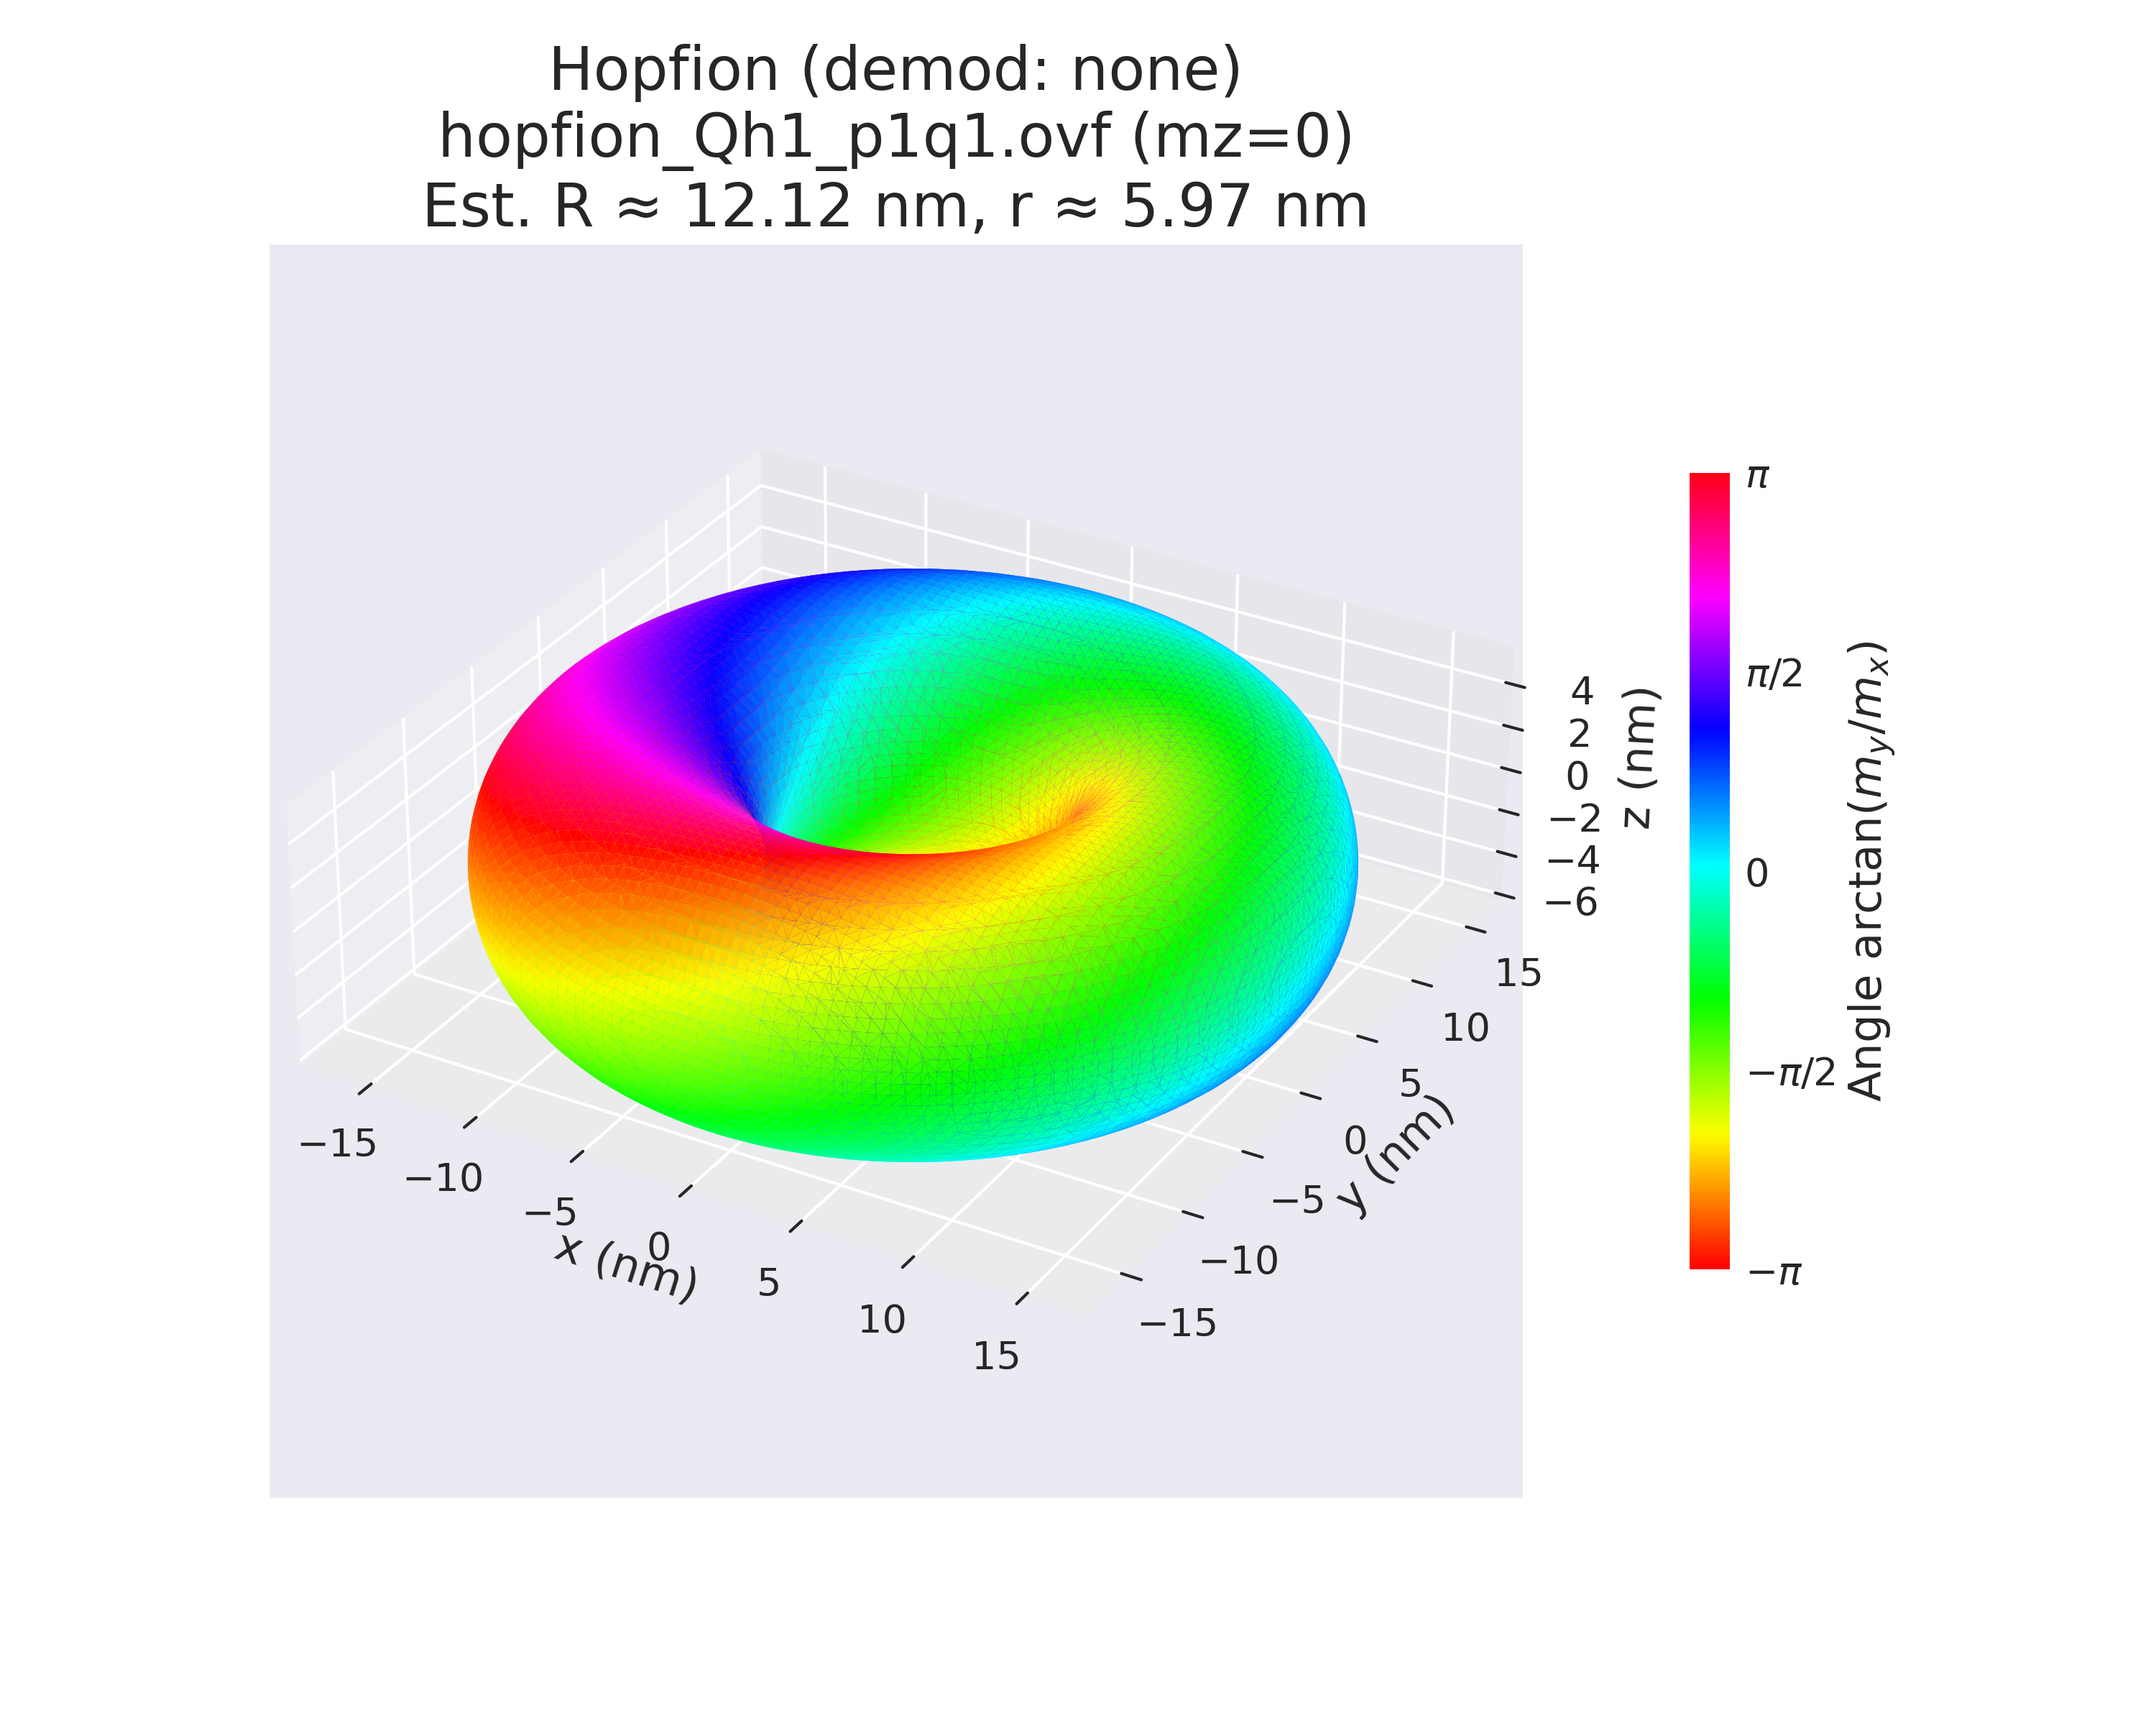
\includegraphics[width=\textwidth]{figures/hopfion_Qh1_p1q1_strategy1.png}
        \caption*{(a) $Q_H=1$ ($p=1, q=1$)}
    \end{minipage}\hfill
    \begin{minipage}{0.48\textwidth}
        \centering
        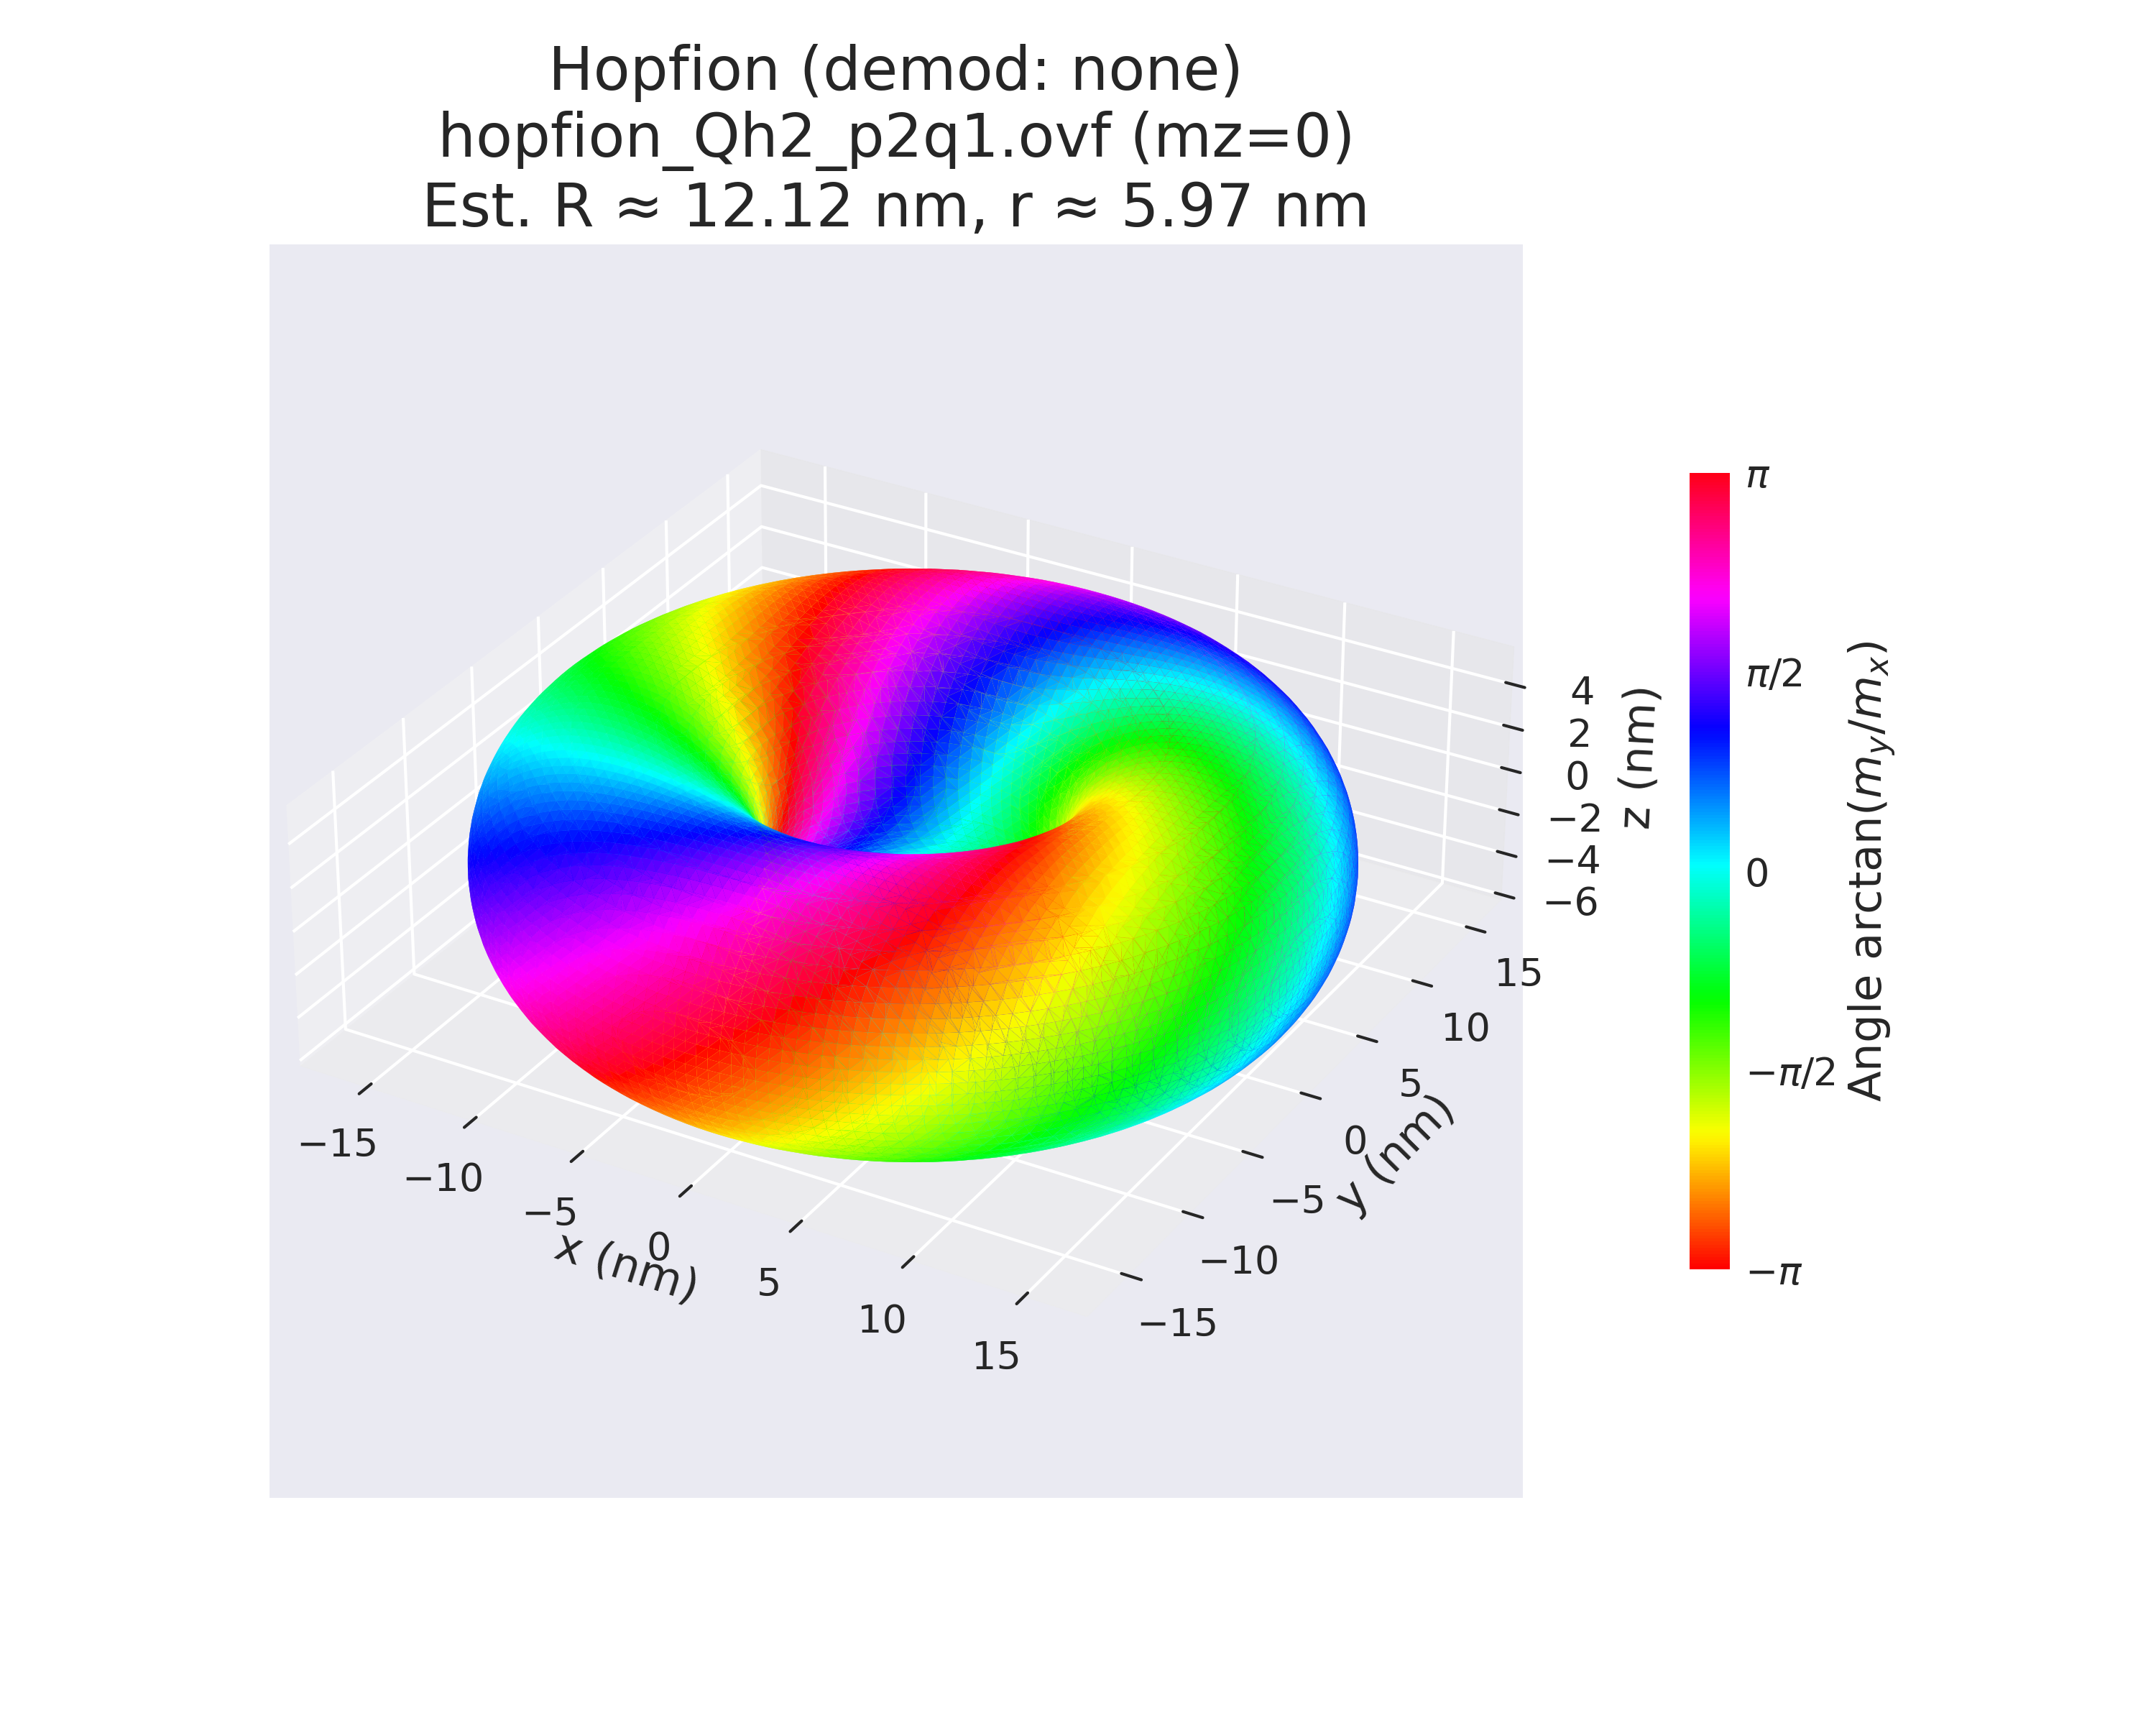
\includegraphics[width=\textwidth]{figures/hopfion_Qh2_p2q1_strategy1.png}
        \caption*{(b) $Q_H=2$ ($p=2, q=1$)}
    \end{minipage}

    \vspace{0.5cm}
    \begin{minipage}{0.48\textwidth}
        \centering
        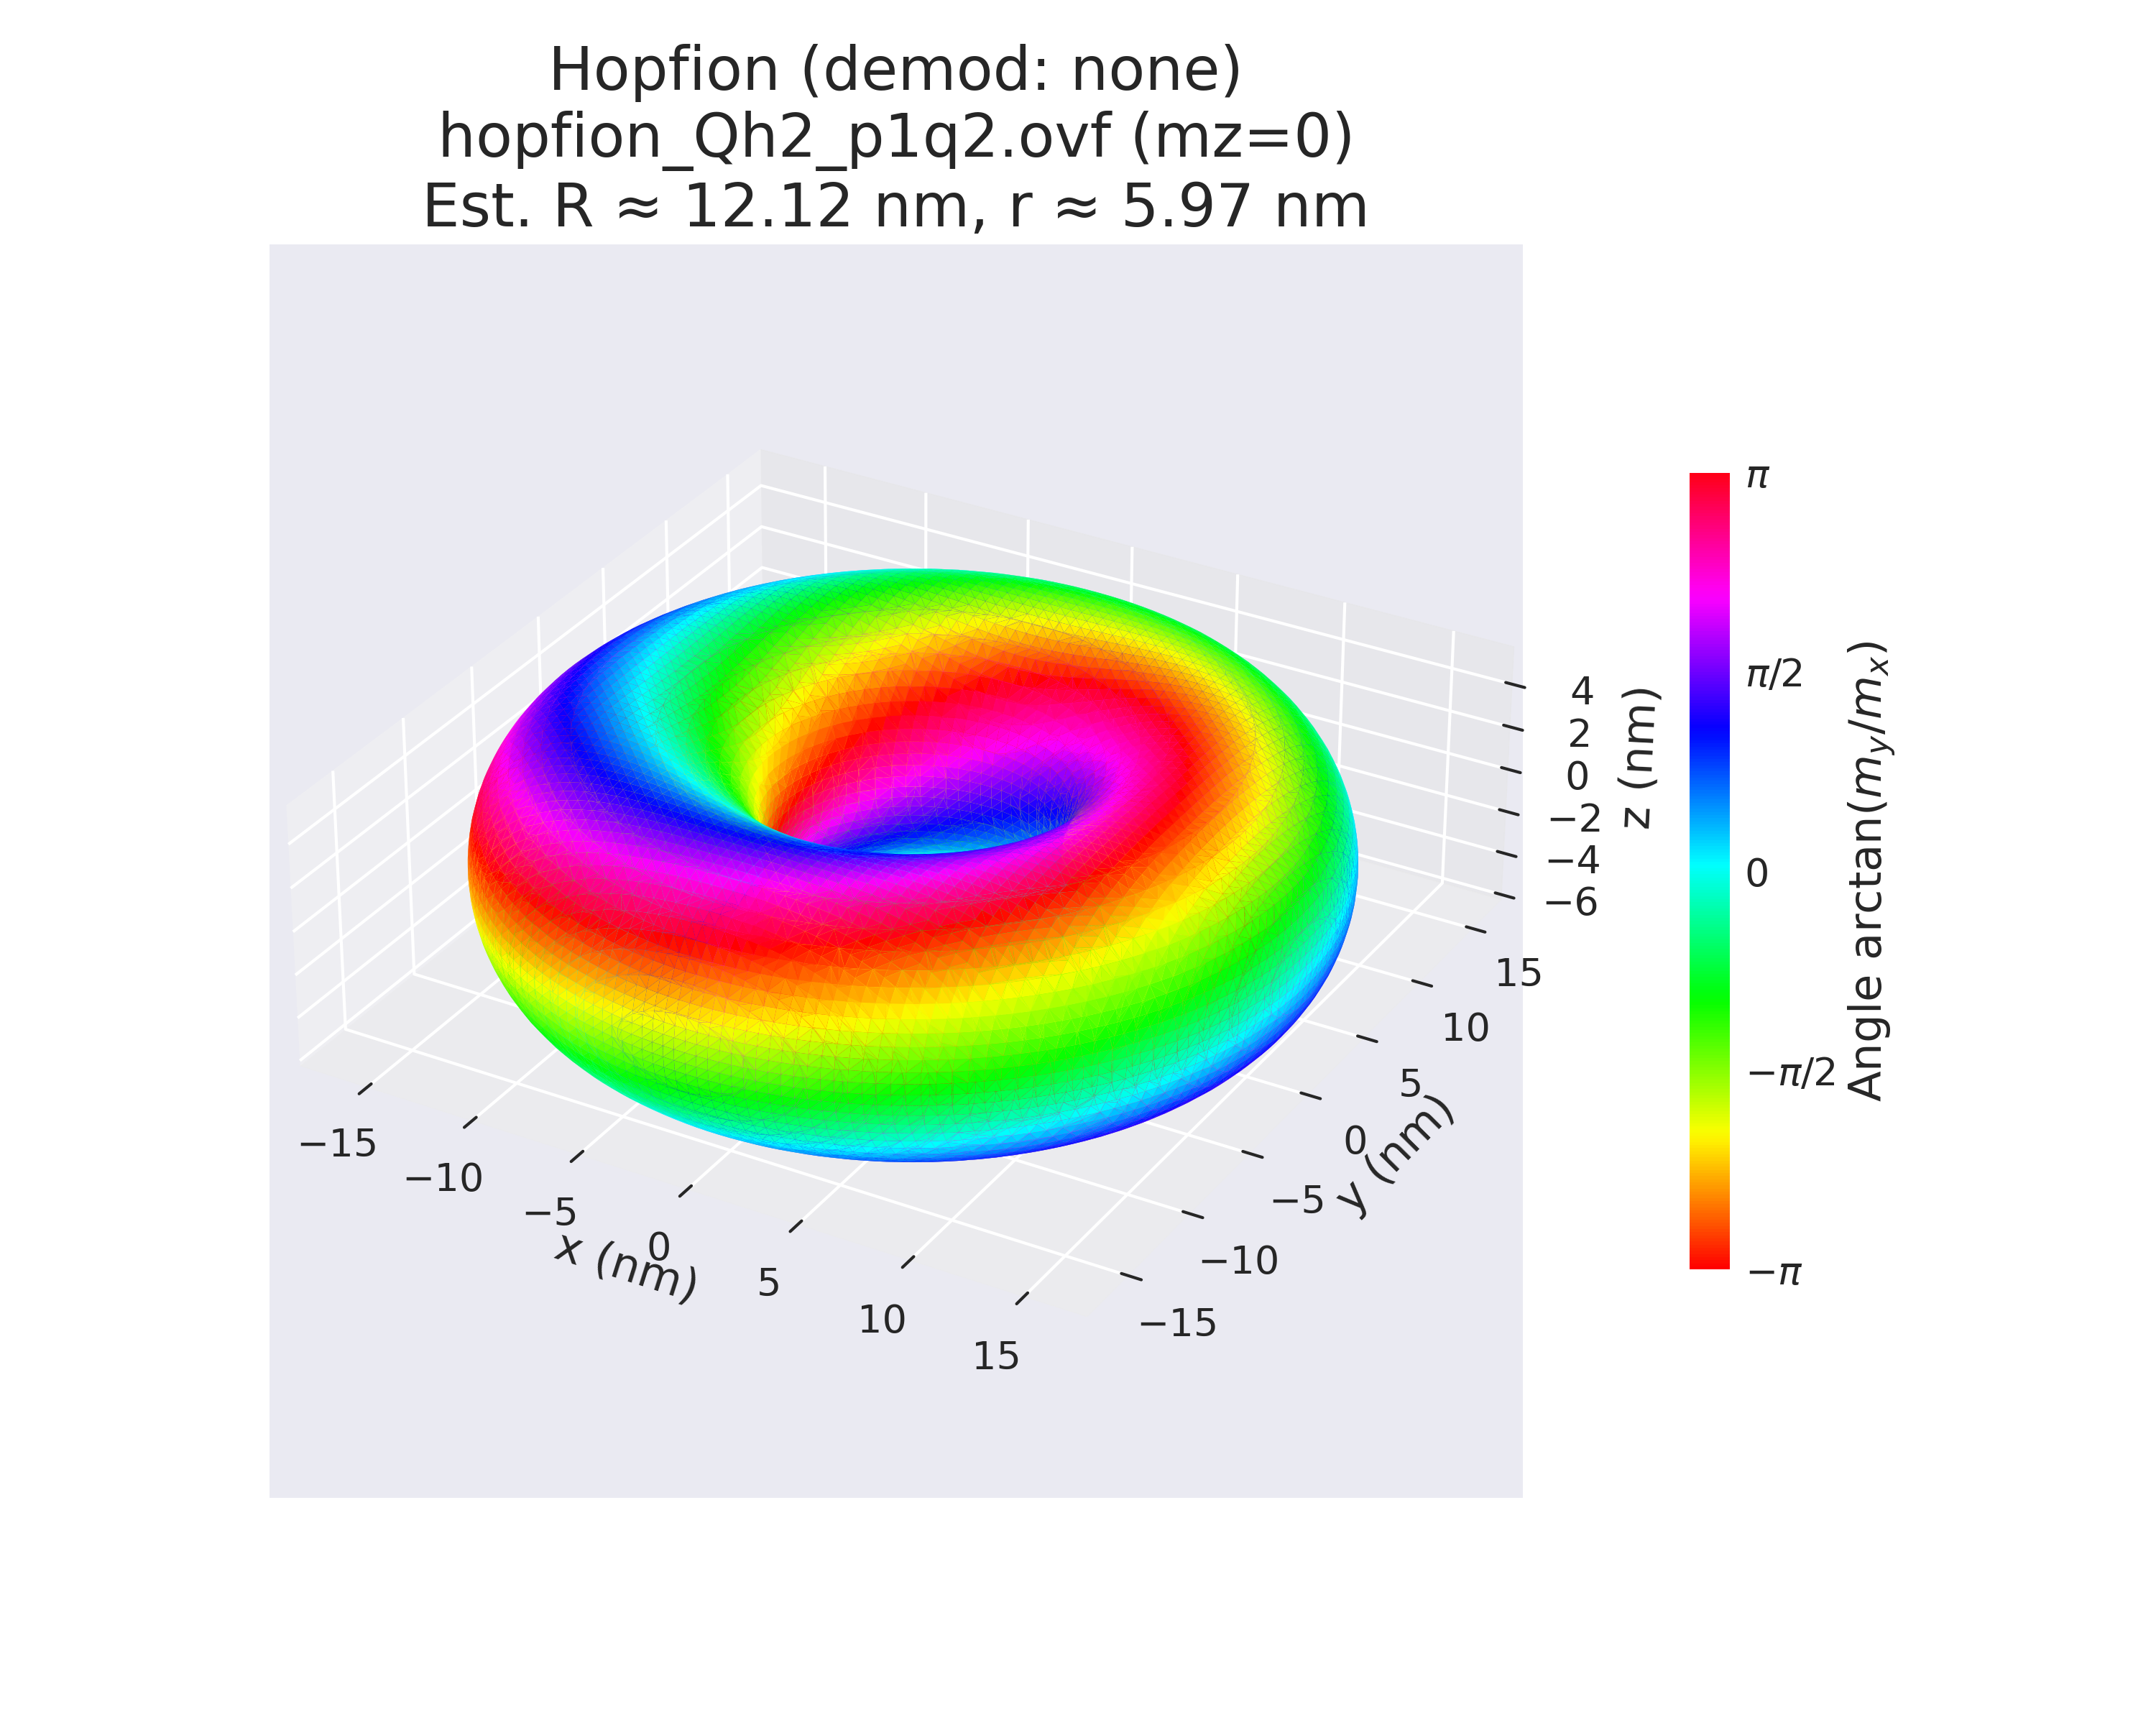
\includegraphics[width=\textwidth]{figures/hopfion_Qh2_p1q2_strategy1.png}
        \caption*{(c) $Q_H=2$ ($p=1, q=2$)}
    \end{minipage}\hfill
    \begin{minipage}{0.48\textwidth}
        \centering
        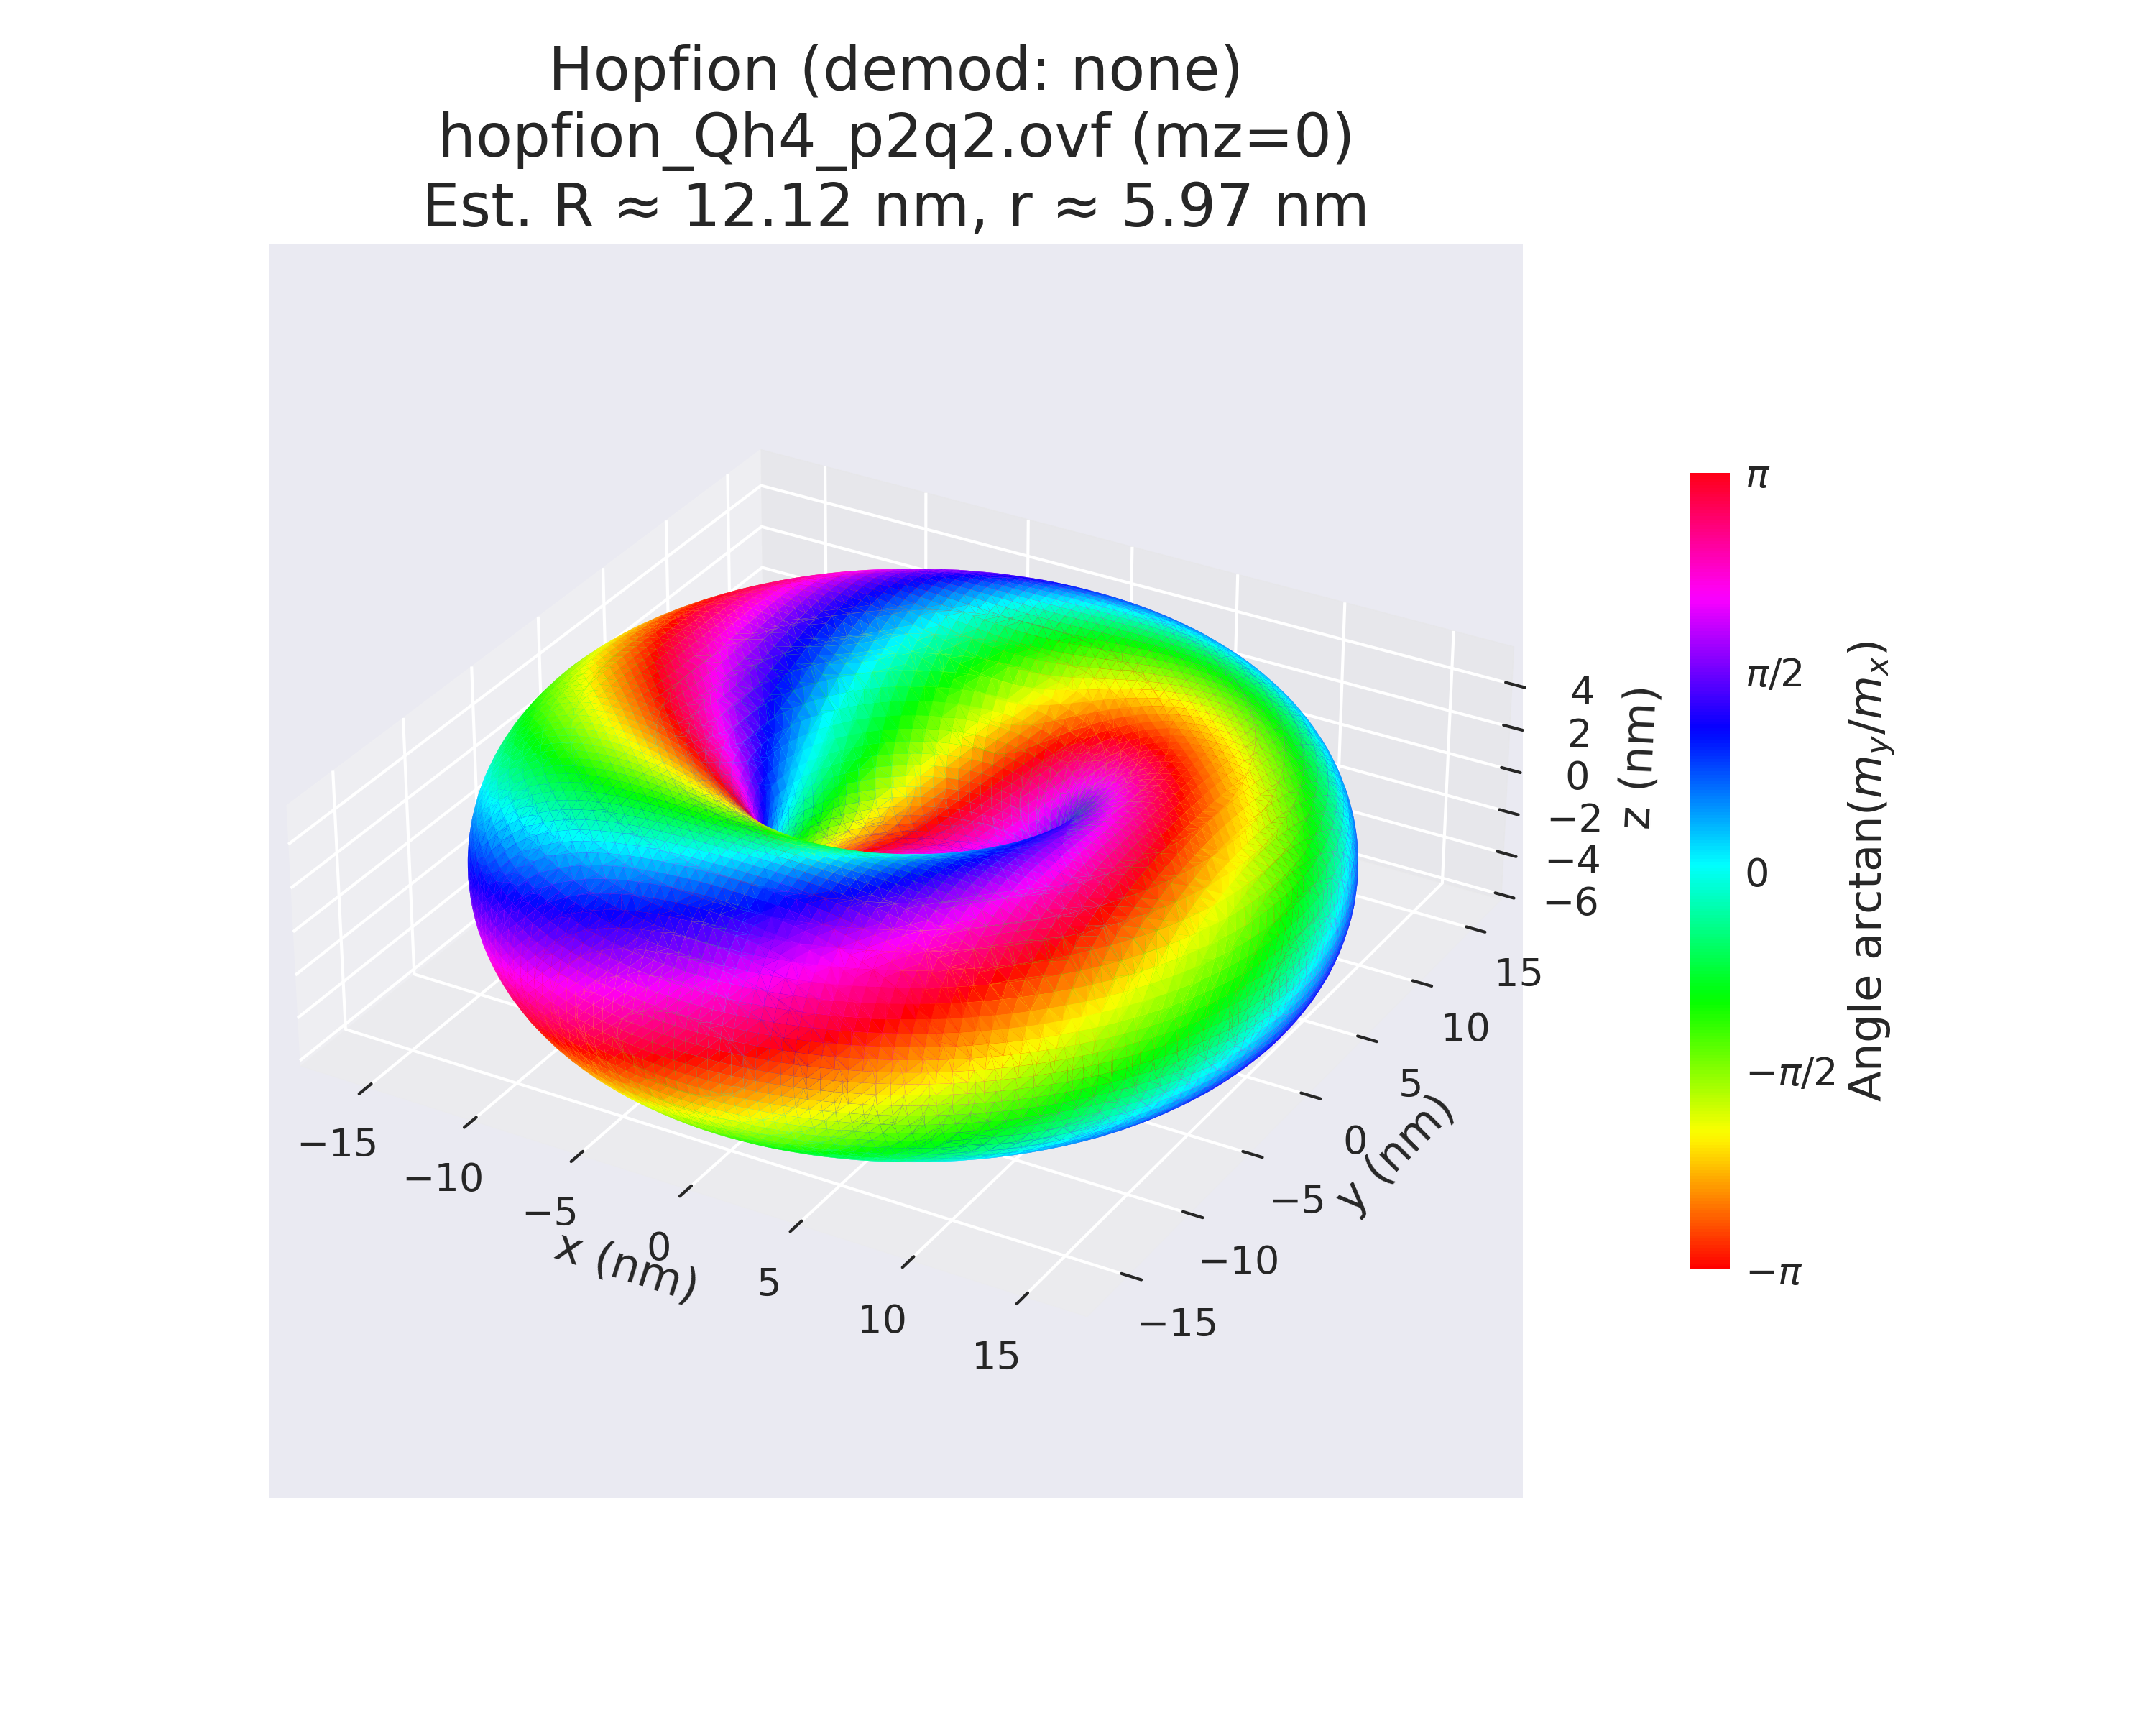
\includegraphics[width=\textwidth]{figures/hopfion_Qh4_p2q2_strategy1.png}
        \caption*{(d) $Q_H=4$ ($p=2, q=2$)}
    \end{minipage}
    \caption{由本文自主开发的离散化生成脚本所构建的不同拓扑荷($Q_H=1, 2, 4$)Hopfion 的三维等值面及其面内相位着色对照。为便于横向比较,四者的理论特征尺寸被统一设定为 $R=\SI{12}{nm}, r=\SI{6}{nm}$。}
    \label{fig:hopfion_vis}
\end{figure}

围绕任意拓扑荷 Hopfion 的初始态构造问题，本章完成了一条从解析框架到可执行工具的完整翻译。理论侧，四元数参数化与环面坐标映射两套既有体系被系统梳理为可编程对象；实现侧，据此落地的 OVF 离散化生成脚本兼容任意 $(p,q)$ 缠绕数，也把反铁磁交替背景纳入可配置项。配套的等值面可视化脚本则凭借自动 AFM 解调与面内相位着色，在几何形貌与矢量分布两个维度上完成了对生成结果的交叉校核。相较于仅能覆盖单一 $Q_H=1$ 构型的传统解析解，本文所构建的这套组合在普适性与灵活性上表现出更明显的优势，为后续章节在稳定性判据与自旋波动力学方面的仿真研究，提供了可直接调用的初始化与分析配套。
